\ifx\allfiles\undefined
\def\pictures{}
\documentclass{XDBAthesis}
\usepackage{todonotes}
\graphicspath{{../figures/}{../omnigraffle/}}
\begin{document}
\else
\fi
\chapter{背景知识}
\label{chap:background}
\section{图基本定义}
\begin{defn}[标号图]\cite{ghash}
    一个可以被四元组$G=(V,E,\Sigma,\lambda)$表示的图称为\emph{标号图(labeled graph)},其中$V$为有限的节点集合,$E$为有限的边集合$\in V\times V$,$\Sigma$是标号集合,$\lambda$是一个标号函数用于给各个节点与边分配标号$\lambda :V\cup E\rightarrow\Sigma$。
\end{defn}
如图\ref{fg:label}就是一个包含六个节点的标号图。需要注意的是标号与标识的区别,标号是图的固有属性,标识只是为了方便使用人为添加的记号。在图\ref{fg:label}中,$v_i $就是标识,而$A,B,C,D$则是标号。

\begin{figure}[htp]
    \begin{minipage}{0.5\textwidth}
        \centering
        \ifx\pictures\undefined
\documentclass{article}
\usepackage{ctex}
\usepackage{tikz}

\begin{document}
\else
\fi
\ifx\hasdraw\undefined
\tikzstyle{vertex}=[circle,draw=black!25,minimum size=20pt,inner sep=0pt]
\tikzstyle{edge} = [draw,thick,-]
\def\hasdraw{}
\fi
    \begin{tikzpicture}[scale=2, auto,swap]
        \foreach \pos/\labels/\name/\lp in {{(0.5,1.5)/1/A/above}, {(1,1)/2/A/above}, {(0,1)/3/B/above},{(0,0)/4/C/left}, {(1,0)/5/C/right},{(2,1)/6/D/above}}
            \node[vertex] (\labels) at \pos [label=\lp:$v_{\labels}$]{$\name$};
        \foreach \source/ \dest  in {1/2,1/3,2/3,2/5,2/4,3/4,3/5,4/5,2/6}
                \path[edge] (\source) --  (\dest);
    \end{tikzpicture}
\ifx\pictures\undefined
\end{document}
\fi
        \figcaption{标号图}
        \label{fg:label}
    \end{minipage}%
    \begin{minipage}{0.5\textwidth}
        \centering
        \ifx\pictures\undefined
\documentclass{article}
\usepackage{ctex}
\usepackage{tikz}
\begin{document}
\else
\fi
\ifx\hasdraw\undefined
\tikzstyle{vertex}=[circle,draw=black!25,minimum size=20pt,inner sep=0pt]
\tikzstyle{edge} = [draw,thick,-]
\def\hasdraw{}
\fi
    \begin{tikzpicture}[scale=2, auto,swap]
        \foreach \pos/\labels/\name/\lp in {{(0.5,1.5)/1/A/above}, {(1,1)/2/A/above}, {(0,1)/3/B/above},{(0,0)/4/C/left}, {(2,1)/5/D/above}}
            \node[vertex] (\labels) at \pos [label=\lp:$v_{\labels}$]{$\name$};
        \foreach \source/ \dest  in {1/2,1/3,2/3,2/4,3/4,2/5}
                \path[edge] (\source) --  (\dest);
    \end{tikzpicture}
\ifx\pictures\undefined
\end{document}
\fi
        \figcaption{图\ref{fg:label}的子图}
        \label{fg:sub}
    \end{minipage}\hfill
\end{figure}
\begin{defn}[子图]
    如果一幅图$G=(V,E,\Sigma,\lambda)$和另一幅图$G'=(V',E',\Sigma',\lambda')$有1-1映射的关系$f:V\rightarrow V'$,那么图$G$就是$G'$的\emph{子图(subgraph)},用$G\in G' $表示。$f$可以有这么几种
\begin{itemize}
    \item 对于所有$v\in V,\lambda(v)=\lambda '(f(v))$
    \item 对于所有$(u,v)\in E,(f(u),f(v))\in E$
    \item 对于所有$(u,v)\in E,\lambda(u,v)=\lambda '(f(u),f(v)) $
\end{itemize}
\end{defn}
换言之,如果一幅图和另一幅图的节点标签,边关系,边标签能一一对应上,那么这副图就是另一幅图的子图。如图\ref{fg:sub}就是图一个\ref{fg:label}的子图,节点标签,边关系及边标签均可一一对应,只有标识可以不同。
\begin{defn}[超图]
    如果图$G$是图$G'$的子图,则$G'$是$G$的\emph{超图}。如对于图\ref{fg:label}和图\ref{fg:sub},图\ref{fg:sub}是图\ref{fg:label}的子图,所以图\ref{fg:label}是图\ref{fg:sub}的超图。
\end{defn}

\begin{defn}[顶点的度]\cite{GraphAlgorithm}
    一个顶点$u$的\emph{度}数是与它相关联的边的数目,记做$degree(u)$。$degree(v_i )=|E(v_i )|,v_i \in V(i=1,2,...,n)$,图\ref{fg:label}中$v_2 $的度$degree(v_2 )=5$,图\ref{fg:sub}中$v_2 $的度为$degree(v_2)=4$。
\end{defn}
\begin{defn}[图的尺寸]\cite{g13}
    一般由图中节点数$|V(G)|$定义。因此图\ref{fg:label}的\emph{尺寸(size)}为6,图\ref{fg:sub}为5。
\end{defn}
\begin{defn}[路径]\cite{GraphAlgorithm}
在图$G(V,E)$中,若从顶点$v_i$出发,沿着一些边经过一些顶点$v_{p1},v_{p2},...,v_{pm}$,到达顶点$v_j $,则称顶点序列$(v_{i},v_{p1},v_{p2},...,v_{pm},v_{j})$为从顶点$v_i $到$v_j $的一条\emph{路径(path)}。如在图\ref{fg:label}中,$(v_{1},v_{2},v_{5})$就是一条$v_1 $到$v_5 $的路径。  
\end{defn}
\begin{defn}[图的同构]\cite{g13}
给定图$g$和图$g'$,若$g'$满足$g'\equiv_{iso}g$,则称$g$与$g'$是\emph{同构图}。$g'\equiv_{iso}g$同构,当且仅当存在一个双射函数$f:V(g)\leftrightarrow V(g')$,其满足下列条件:
\begin{itemize}
    \item 对于所有$v\in V,\lambda(v)=\lambda '(f(v))$
    \item 对于所有$u,v\in V,(u,v)\in E\Leftrightarrow (f(u),f(v))\in E$
    \item 对于所有$(u,v)\in E,\lambda(u,v)=\lambda '(f(u),f(v)) $
\end{itemize}  
\end{defn}
如图\ref{fg:iso},图$G_1$和图$G_2$就是一组同构图,顶点标号$A\leftrightarrow X,B\leftrightarrow Y,C\leftrightarrow Z$,$G_1$中的边与$G_2$的边也形成双射关系
\begin{figure}[htb]
    \centering
    \subfigure[$G_1$]{
        \ifx\pictures\undefined
\documentclass{article}
\usepackage{ctex}
\usepackage{tikz}
\begin{document}
\else
\fi
\ifx\hasdraw\undefined
\tikzstyle{vertex}=[circle,draw=black!25,minimum size=20pt,inner sep=0pt]
\tikzstyle{edge} = [draw,thick,-]
\def\hasdraw{}
\fi
\begin{tikzpicture}[scale=0.5, auto,swap]
    \foreach \pos/\labels/\name/\where in {{(3,6)/1/A/right}, {(0,3.5)/2/B/above}, {(1,0)/3/C/left},{(5,0)/4/A/right}, {(6,3.5)/5/B/above}}
        \node[vertex] (\labels) at \pos [label=\where:$v_{\labels}$]{$\name$};
    \foreach \source/ \dest  in {1/2,2/3,3/4,4/5,5/1}
            \path[edge] (\source) --  (\dest);
\end{tikzpicture}
\ifx\pictures\undefined
\end{document}
\fi
    }
    \subfigure[$G_2$]{
        \ifx\pictures\undefined
\documentclass{article}
\usepackage{ctex}
\usepackage{tikz}
\begin{document}
\else
\fi
\ifx\hasdraw\undefined
\tikzstyle{vertex}=[circle,draw=black!25,minimum size=20pt,inner sep=0pt]
\tikzstyle{edge} = [draw,thick,-]
\def\hasdraw{}
\fi
\begin{tikzpicture}[scale=0.5, auto,swap]
    \foreach \pos/\labels/\name/\where in {{(3,6)/1/X/right}, {(0,3.5)/2/X/above}, {(1,0)/3/Y/left},{(5,0)/4/Y/right}, {(6,3.5)/5/Z/above}}
        \node[vertex] (\labels) at \pos [label=\where:$v_{\labels}$]{$\name$};
    \foreach \source/ \dest  in {1/3,2/4,3/5,4/1,5/2}
            \path[edge] (\source) --  (\dest);
\end{tikzpicture}
\ifx\pictures\undefined
\end{document}
\fi
    }
    \caption{图的同构}
    \label{fg:iso}
\end{figure}

\section{图存储表示方式}
图存储表示方法有很多种,常用的有2种:\emph{邻接矩阵(Adjacency Matrix)}和\emph{邻接表(Adjacency List)}。本节还将介绍一种新颖的图表示方法\emph{简化包表示(Reduced Bag Representation)}\cite{ghash}。
\subsection{邻接矩阵}
 在邻接矩阵存储方法中,除了一个记录各个顶点信息的顶点数组外,还有一个表示各个顶点之间关系的矩阵,称为\emph{邻接矩阵}\cite{GraphAlgorithm},设$G(V,E)$是一个具有$n$个顶点的图,则图的邻接矩阵是一个$n\times n$的二维数组,用$Edge[n][n]$表示,定义为:
\begin{equation}
    Edge[i][j]=\left\{
    \begin{aligned}
        1 & , if (i,j)\in E \\
        0 & , else    
    \end{aligned}\right. 
\end{equation}

%\todo{增加邻接矩阵图} 

\subsection{邻接表}
    \emph{邻接表}\cite{GraphAlgorithm}就是将同一个顶点发出的边连接在同一个称为边链表的单链表中。边链表的每个节点代表一条边,称为边节点。每个边节点有两个域:该边终点的序号以及下一个边节点的指针。
    
%\todo{增加邻接表图}   
%    \begin{figure}[htb]
%        \centering
%        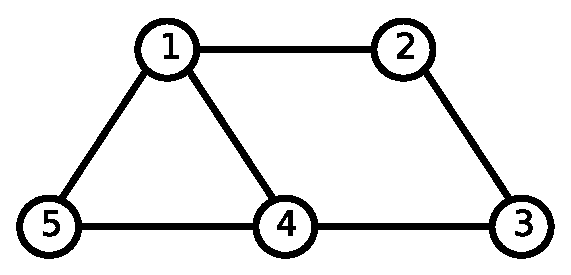
\includegraphics[width=0.4\textwidth]{../figures/BasicGraph_GraphExample}
%        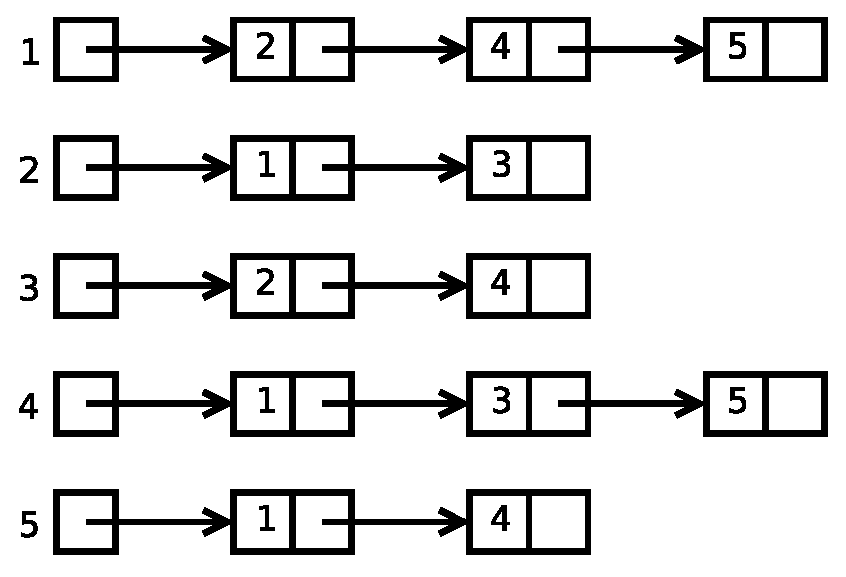
\includegraphics[width=0.4\textwidth]{../figures/BasicGraph_AdjacencyListRepresentation}
%        \caption{邻接表}
%        \label{fg:adjacencyList}
%    \end{figure}
\subsection{包表示法}
\emph{包表示法}是Wang教授等人在\emph{G-Hash}\cite{ghash}中提出的一种方法。这种方法的主要思想是将图中的各个节点特征提取出来形成一个列表,然后将这些特征就作为每个节点的标识。这样整幅图就变成了一个字符串的包,也就是一组字符串。通常,我们用这个节点的标号和其邻接节点的不同标号数目为特征。例\ref{exmp:bag1}所示就是一个常用的包表示方法
\begin{exmp}
    表\ref{tb:bagr1}是图\ref{fg:label}的包表示。我们以节点标号和其邻接节点各个标号的个数作为特征,因此有五个特征:本身标号,A,B,C,D分别的个数。所以加上第一列的标识,表一共有六列。而一共有六个不同节点,所以有六行。我们以$v_3 $为例,详细说明下抽取特征的步骤。首先$v_3 $的标号是B,所以Label为B,然后和$v_3$邻接的共有四个节点,分别是$v_1 ,v_2 ,v_4 ,v_5 $,其标号分别为$A,A,C,C$所以$\#A=2,\#C=2$其余为0。节点$v_3 $的包表示就是“B,2,0,2,0”,如表\ref{tb:bagr1}所示。需要注意一点的是,包表示不仅仅这一种表示方法,对于选取什么样的特征并没有限制。不过特征必须是离散的,这样才可以用字符串表示。
    \label{exmp:bag1}
\end{exmp}


\begin{table}[htb]
    \centering
    \begin{tabular}{c|c|c|c|c|c}
        Nodes & Label & \#A & \#B & \#C & \#D \\ \hline
        $v_1$ & A & 1 & 1 & 0 & 0 \\ \hline
        $v_2$ & A & 1 & 1 & 2 & 1 \\ \hline
        $v_3$ & B & 2 & 0 & 2 & 0 \\ \hline
        $v_4$ & C & 1 & 1 & 1 & 0 \\ \hline
        $v_5$ & C & 1 & 1 & 1 & 0 \\ \hline
        $v_6$ & D & 1 & 0 & 0 & 0 \\ \hline
    \end{tabular}
    \tabcaption{图\ref{fg:label}的包表示}
    \label{tb:bagr1}
\end{table}
    
\section{图查询类型}
根据图之间的包含关系,可将图查询分为子图查询和超图查询;根据图查询的精确程度,可以将其分为精确查询和相似查询\cite{g13}。
\begin{defn}[子图查询]\cite{FSD}
子图查询的问题为:对于给定的一个查询图,返回图数据库中所有查询图的超图。给定一个图数据库$GD$和一个查询图$q$,子图查询的目的是找出在$GD$中所有包含$q$或者$q$的同构的图的集合,最后返回该超图集合$Q$。$Q={g|g\in GD\wedge q\subseteq g}$。
\end{defn}
\begin{defn}[超图查询]\cite{ssosc}
超图查询的问题为:对于给定的一个查询图,返回图数据库中所有查询图的子图。给定一个图数据库$GD$和一个查询图$q$,超图查询的目的是找出在$GD$中所有以$q$为超图的图的集合,最后返回该子图集合$Q$。$Q={g|g\in GD\wedge q\supseteq g}$。    
\end{defn}

\begin{figure}[htb]
    \centering
    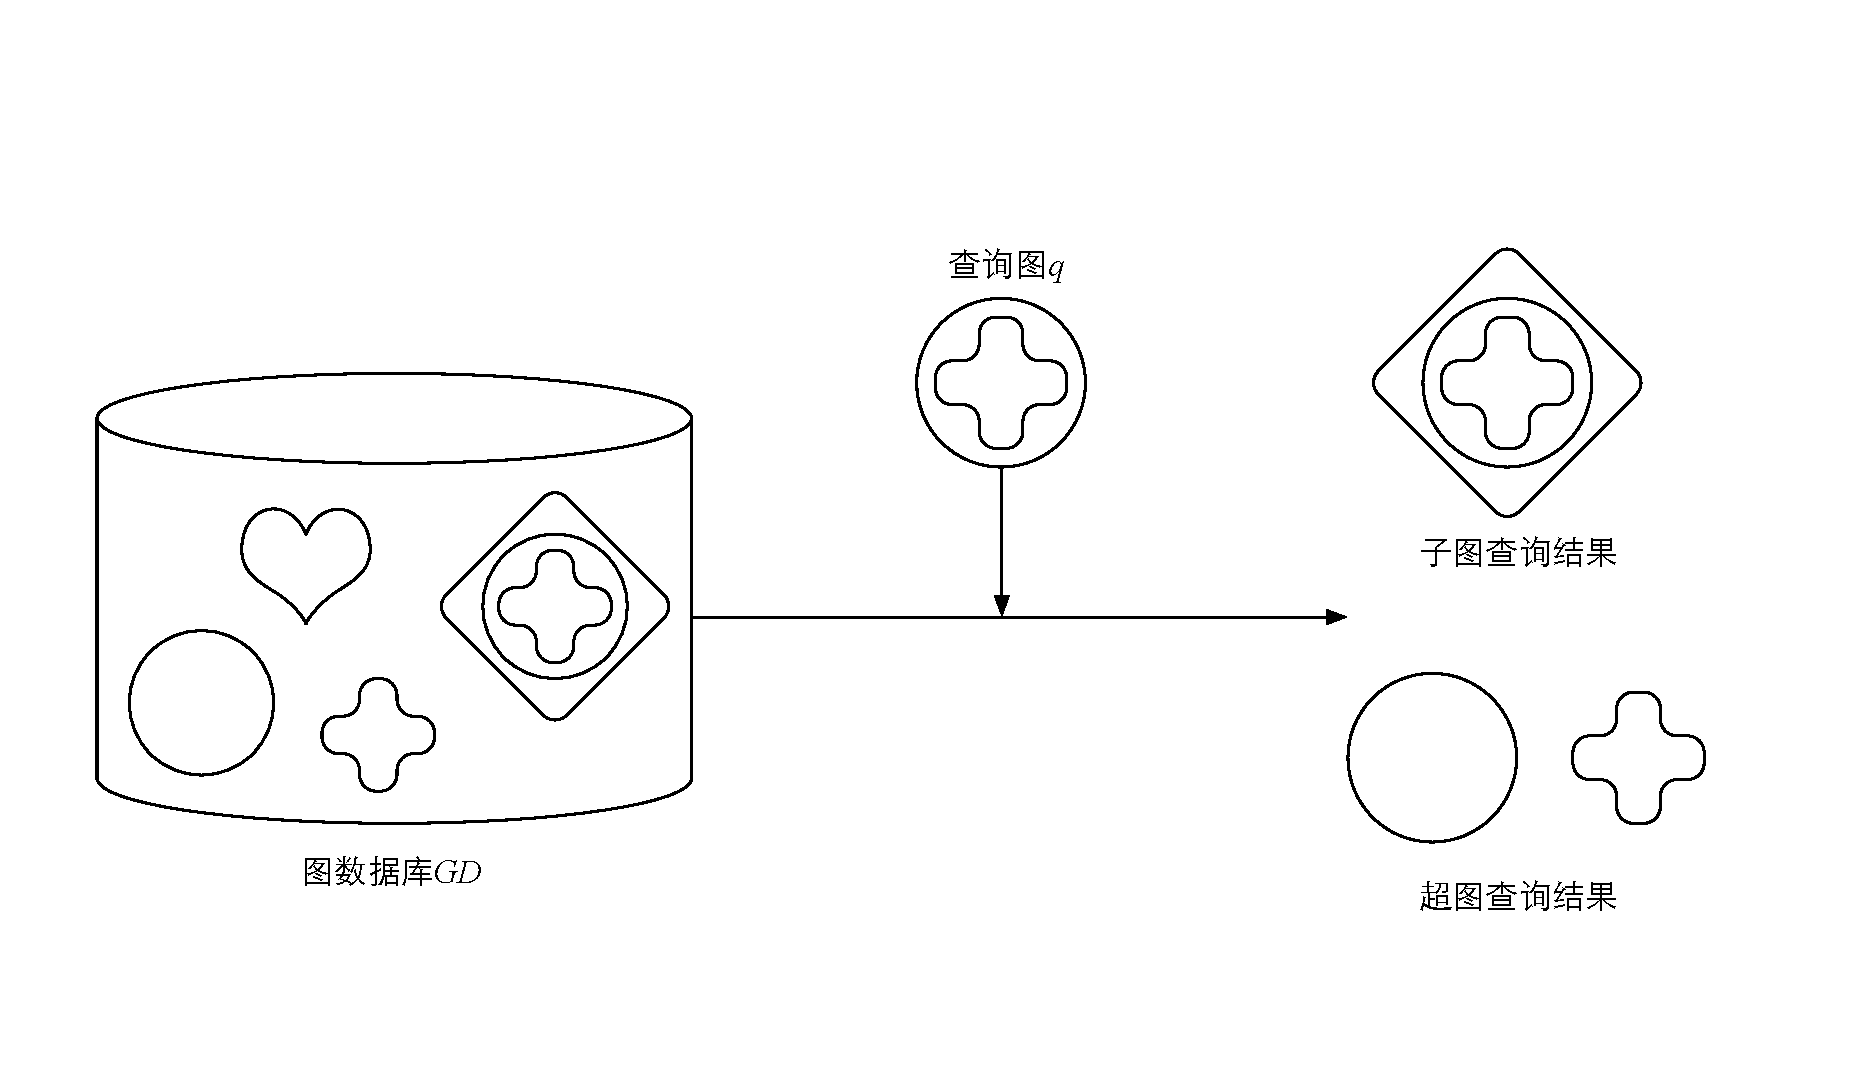
\includegraphics[width=0.75\textwidth]{Database.eps}
    \caption{子图查询与超图查询}
    \label{fg:subsup}
\end{figure}

图\ref{fg:subsup}就是同一个查询$q$在同一数据库中子图查询和超图查询的不同结果。



\begin{defn}[精确查询]\cite{gIndex}
图精确查询的问题是这样定义的:对于给定数据库$G={g_1 ,g_2 ,...,g_n }$,查询图$q$,返回$G$中与$q$具有子图同构的图集合。具体可以分为子图查询和超图查询。如图\ref{fg:simacu}所示,对于精确查询查询图$q$的结果就是$G_1 ,G_2 $
\end{defn}


\begin{defn}[近似查询]\cite{gghash}
图近似查询,又称相似性搜索,是这样定义的:对于给定数据库$G={g_1 ,g_2 ,...,g_n }$,查询图$q$,返回$G$中与$q$距离小于预设阀值的图集合。如图\ref{fg:simacu}所示,对于近似查询查询图$q$的结果就是$G_1 ,G_2 ,G_3 ,G_4 $
\end{defn}

因此,近似查询中相似性度量方法和预设的阀值决定了结果集的大小。阀值越大,结果集越大;阀值越小,结果集越少。当阀值为零是,其结果应该与精确查询一致。

\begin{figure}[htb]
    \centering
    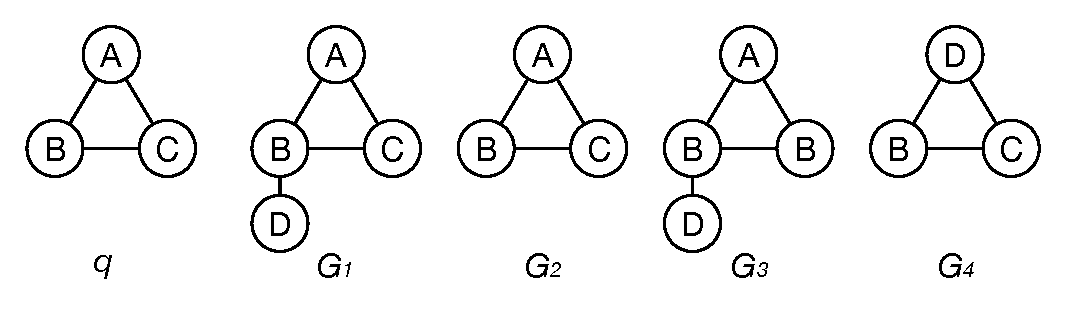
\includegraphics[width=0.8\textwidth]{2last}
    \caption{精确查询与相似查询}
    \label{fg:simacu}
\end{figure}

常见的相似性度量方法有两种,一种方法是\emph{编辑距离(edit distance)}.\emph{编辑距离}就是我们将图$G$通过一系列操作(如增删点边,重新标号等)变换为另一个图$G^{'}$所需的操作数。我们可以通过给不同操作分配不同的权值,然后计算权值和作为距离,这样可以让距离更为符合我们实际需求。虽然编辑距离是一种非常直观的图相似性测度方法,但是我们很难计算(实际上,这是个NP-hard问题)。还有一种方法是\emph{最大公共子图(maximal common subgraph)}\cite{mcs},这里就不详细说明了。

\ifx\allfiles\undefined
%\renewcommand\refname{参考文献}
\bibliographystyle{unsrt}
\bibliography{main}
\end{document}
\fi